\documentclass[12pt]{article}

\usepackage[a4paper, total={6in, 8in}]{geometry}
\usepackage{graphicx}
\usepackage{subcaption}
\graphicspath{ {./imgs/} }
\usepackage{xurl}
\usepackage{hyperref}
\hypersetup{
    colorlinks=true,
    linkcolor=,
    urlcolor=blue,
    pdftitle={Overleaf Example},
    pdfpagemode=FullScreen,
}

\title{Palazzo di Giustizia di Milano}
\author{Eugenio Barbieri Viale}
\date{}

\begin{document}
\setlength{\parindent}{0pt}
\maketitle

\tableofcontents
\newpage

\section{Informazioni}
\begin{itemize}
  \item Tipologia: \textit{Palazzo, tribunale}
  \item Posizione: \textit{Corso di Porta Vittoria}
  \item Movimento: \textit{Monumentalismo fascista}
  \item Periodo di costruzione: \textit{1932 - 1940}
  \item Architetto: \textit{Marcello Piacentini}
  \item Committenza: \textit{Comune di Milano}
  \item Altri artisti: \textit{Mario Sironi, Carlo Carrà, Attilio Selva, Romano Romanelli}
  \item Area: \textit{30.000 m²}
\end{itemize}

\newpage
\section{Storia}
\subsection{Palazzo del Capitano di Giustizia}
L'edificio, situato in \textit{piazza Cesare Beccaria}, fu costruito tra il 1570 e il 1605 e fu finanziato da \textit{Carlo Borromeo}. Denominato dal popolo milanese come \textit{"l'alberg di do compann"} per le sue due campane, tra gli anni 1870 e 1880 si cominciò a lamentare l'ineguatezza del palazzo come sede di giustizia. \\
Le proposte e i progetti furono innumerevoli, ma si dovettero aspettare quarant'anni per trovare una soluzione. Intorno agli anni '20 fu infatti disposto il trasferimento della caserma di polizia di \textit{Santa Prassede} situatata in \textit{corso di Porta Vittoria}, fatta realizzare da \textit{Radetzky} al posto dell'omonimo monstero. \\
In quest'area, estesa circa quanto l'attuale \textit{piazza Duomo}, si decise di edificare il futuro Palazzo di Giustizia di Milano.

\subsection{Concorso}
Il 22 aprile del 1929 (anno VIII) il Comune di Milano bandisce il concorso per il progetto del nuovo Palazzo di Giustizia di Milano. Il 4 novembre la giuria che dovrà provvedere all'assegnazione del progetto si riunisce in una sala del Politecnico. Viene convocata dal Podestà, il quale invita la giuria a \textit{"procedere nei lavori con la fascistica elasticità che il ritmo della nuova vita italiana
impone"}. \\
I progetti presentati sono 11, dei quali 5 vengono scartati. La giuria si riunirà in 4 sedute, ma non riuscirà a individuare un vincitore. Non viene quindi assegnato un primo premio, mentre il secondo premio viene conferito al progetto \textit{"Bianco, rosso e nero"} e il terzo al progetto \textit{"Ruit hora"}. Il 18 aprile 1930 il Podestà \textit{Marcello Visconti di Modrone} viene invitato dalla giuria a scegliere un architetto di sua preferenza. \\
Così, un anno dopo la pubblicazione del bando, l'incarico viene affidato a \textit{Marcello Piacentini}. \\
Tra le 29 ditte invitate alla licitazione privata, di cui 27 con sede a Milano, risulta vincitrice una ditta di Genova.

\section{Analisi distributiva}
\subsection{Pianta}
% 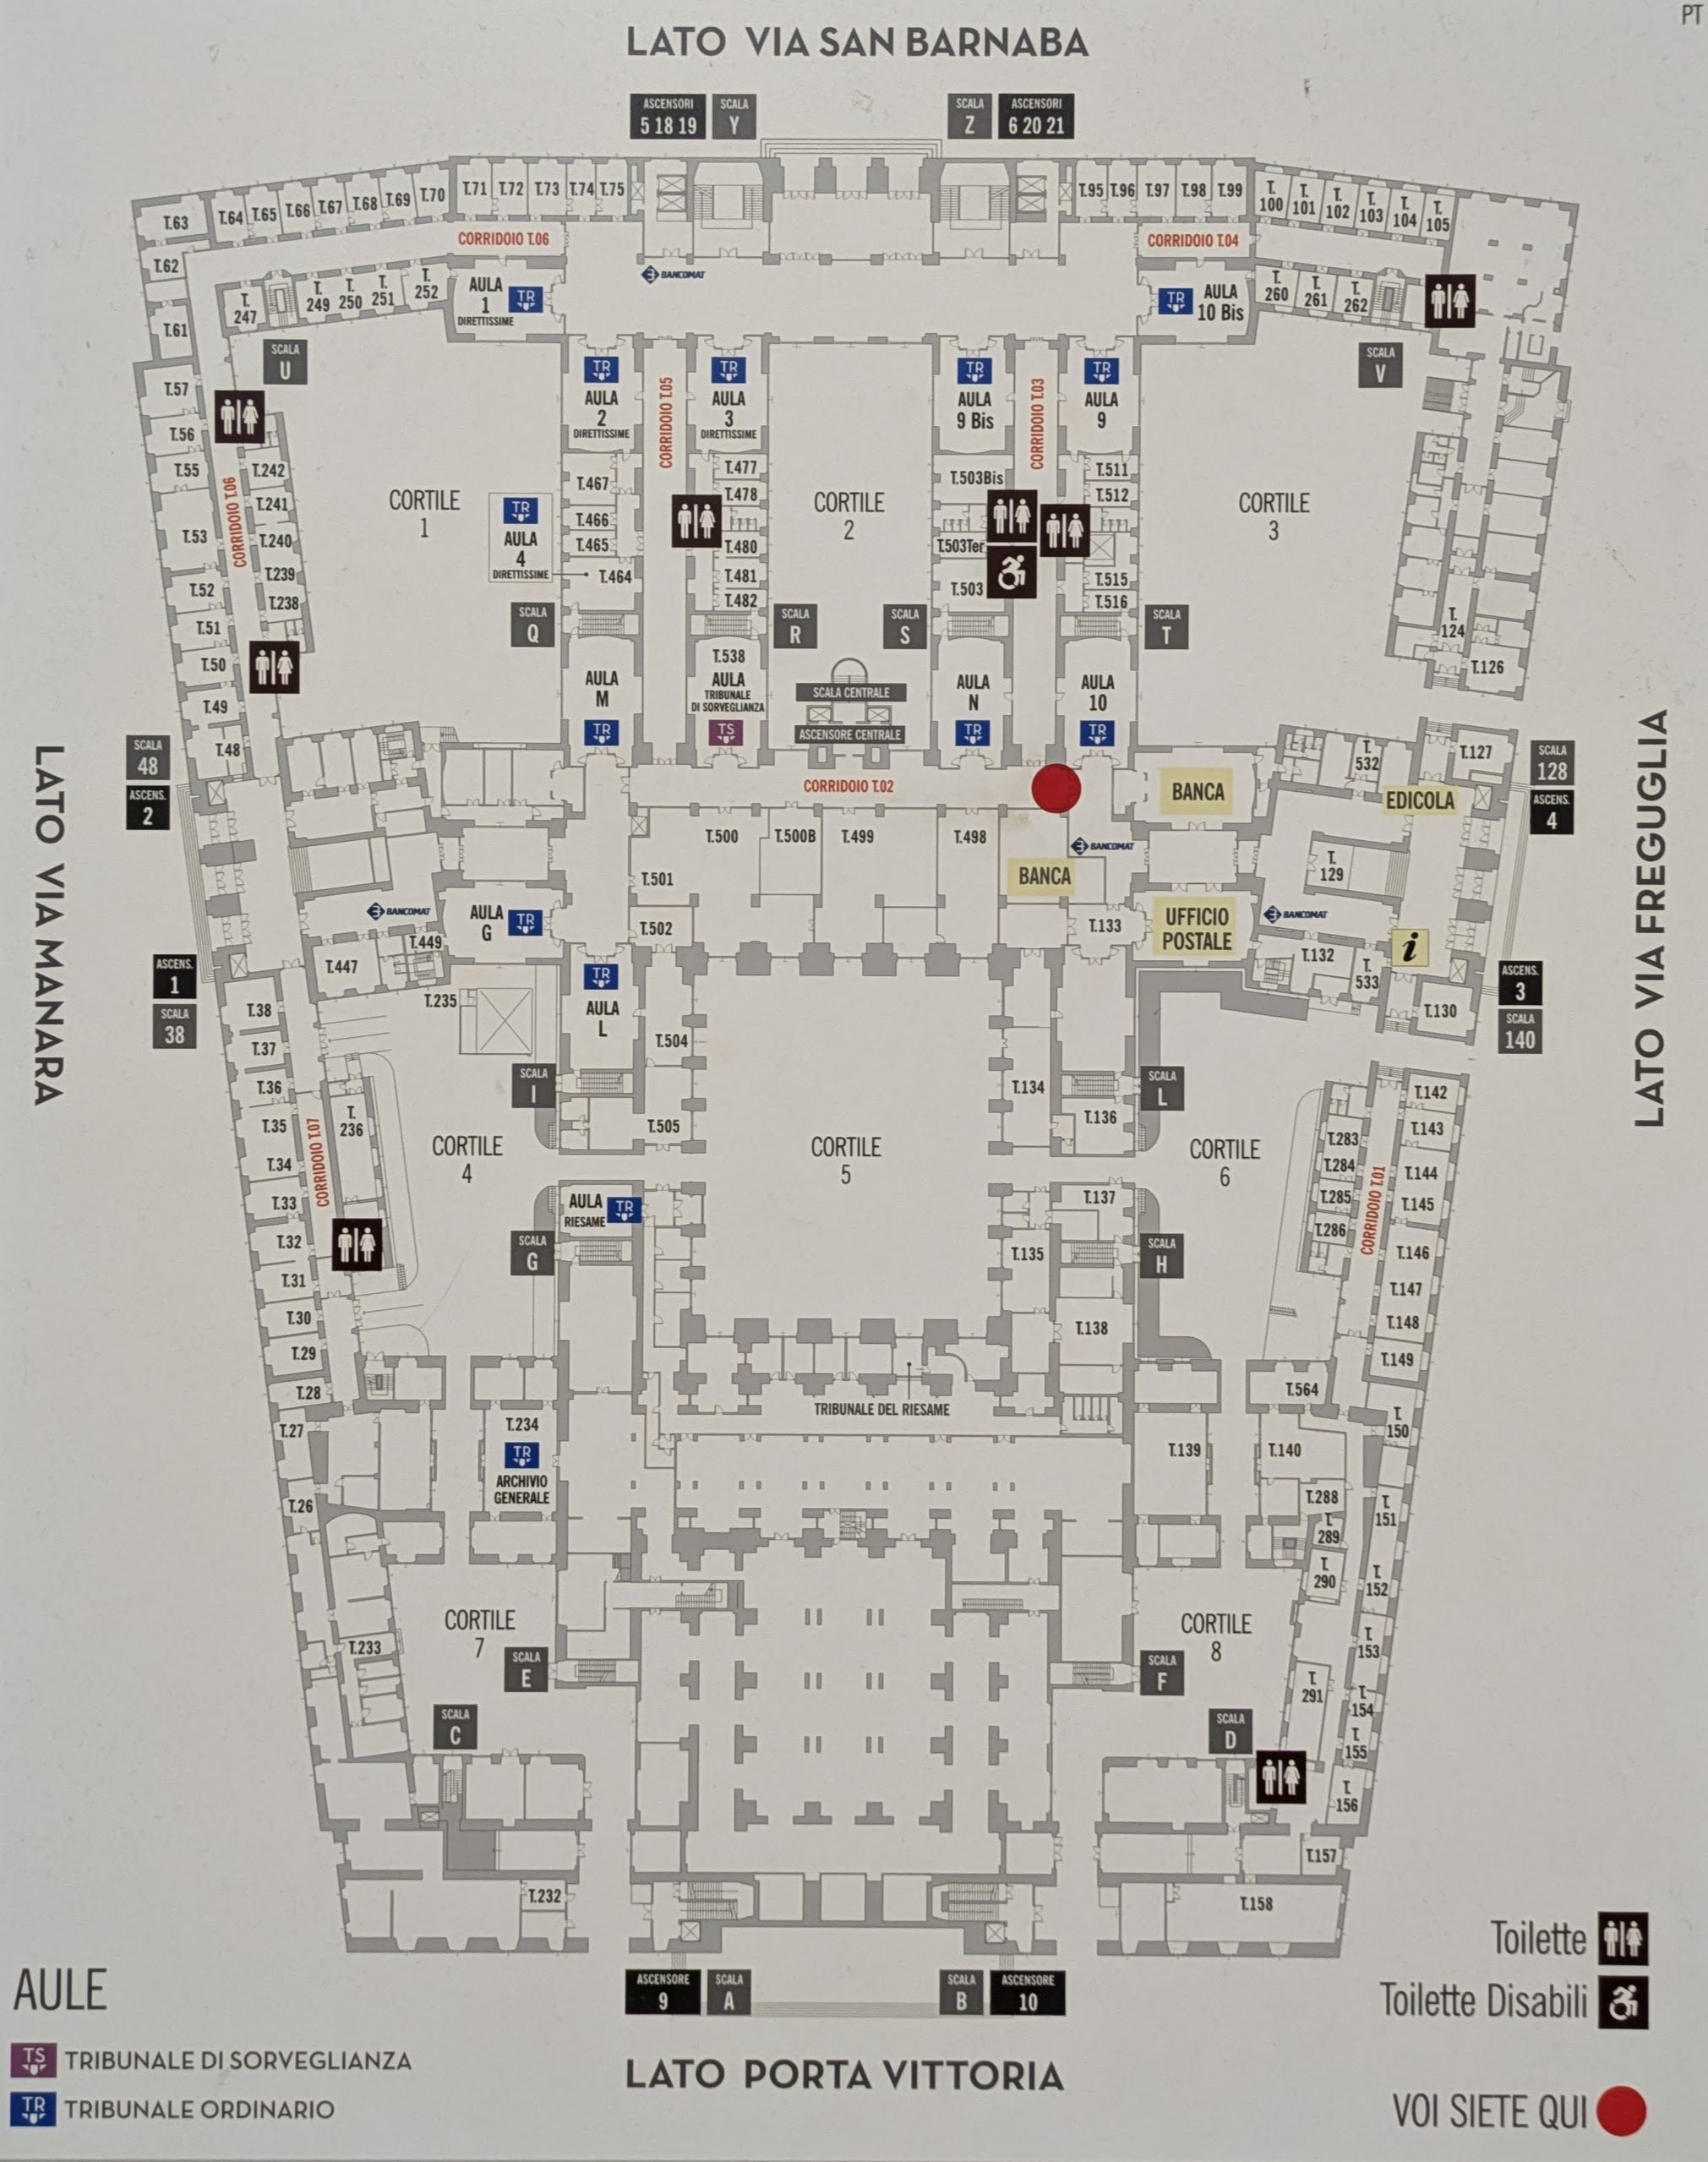
\includegraphics[width=\textwidth]{pianta.jpg}
\begin{center}
  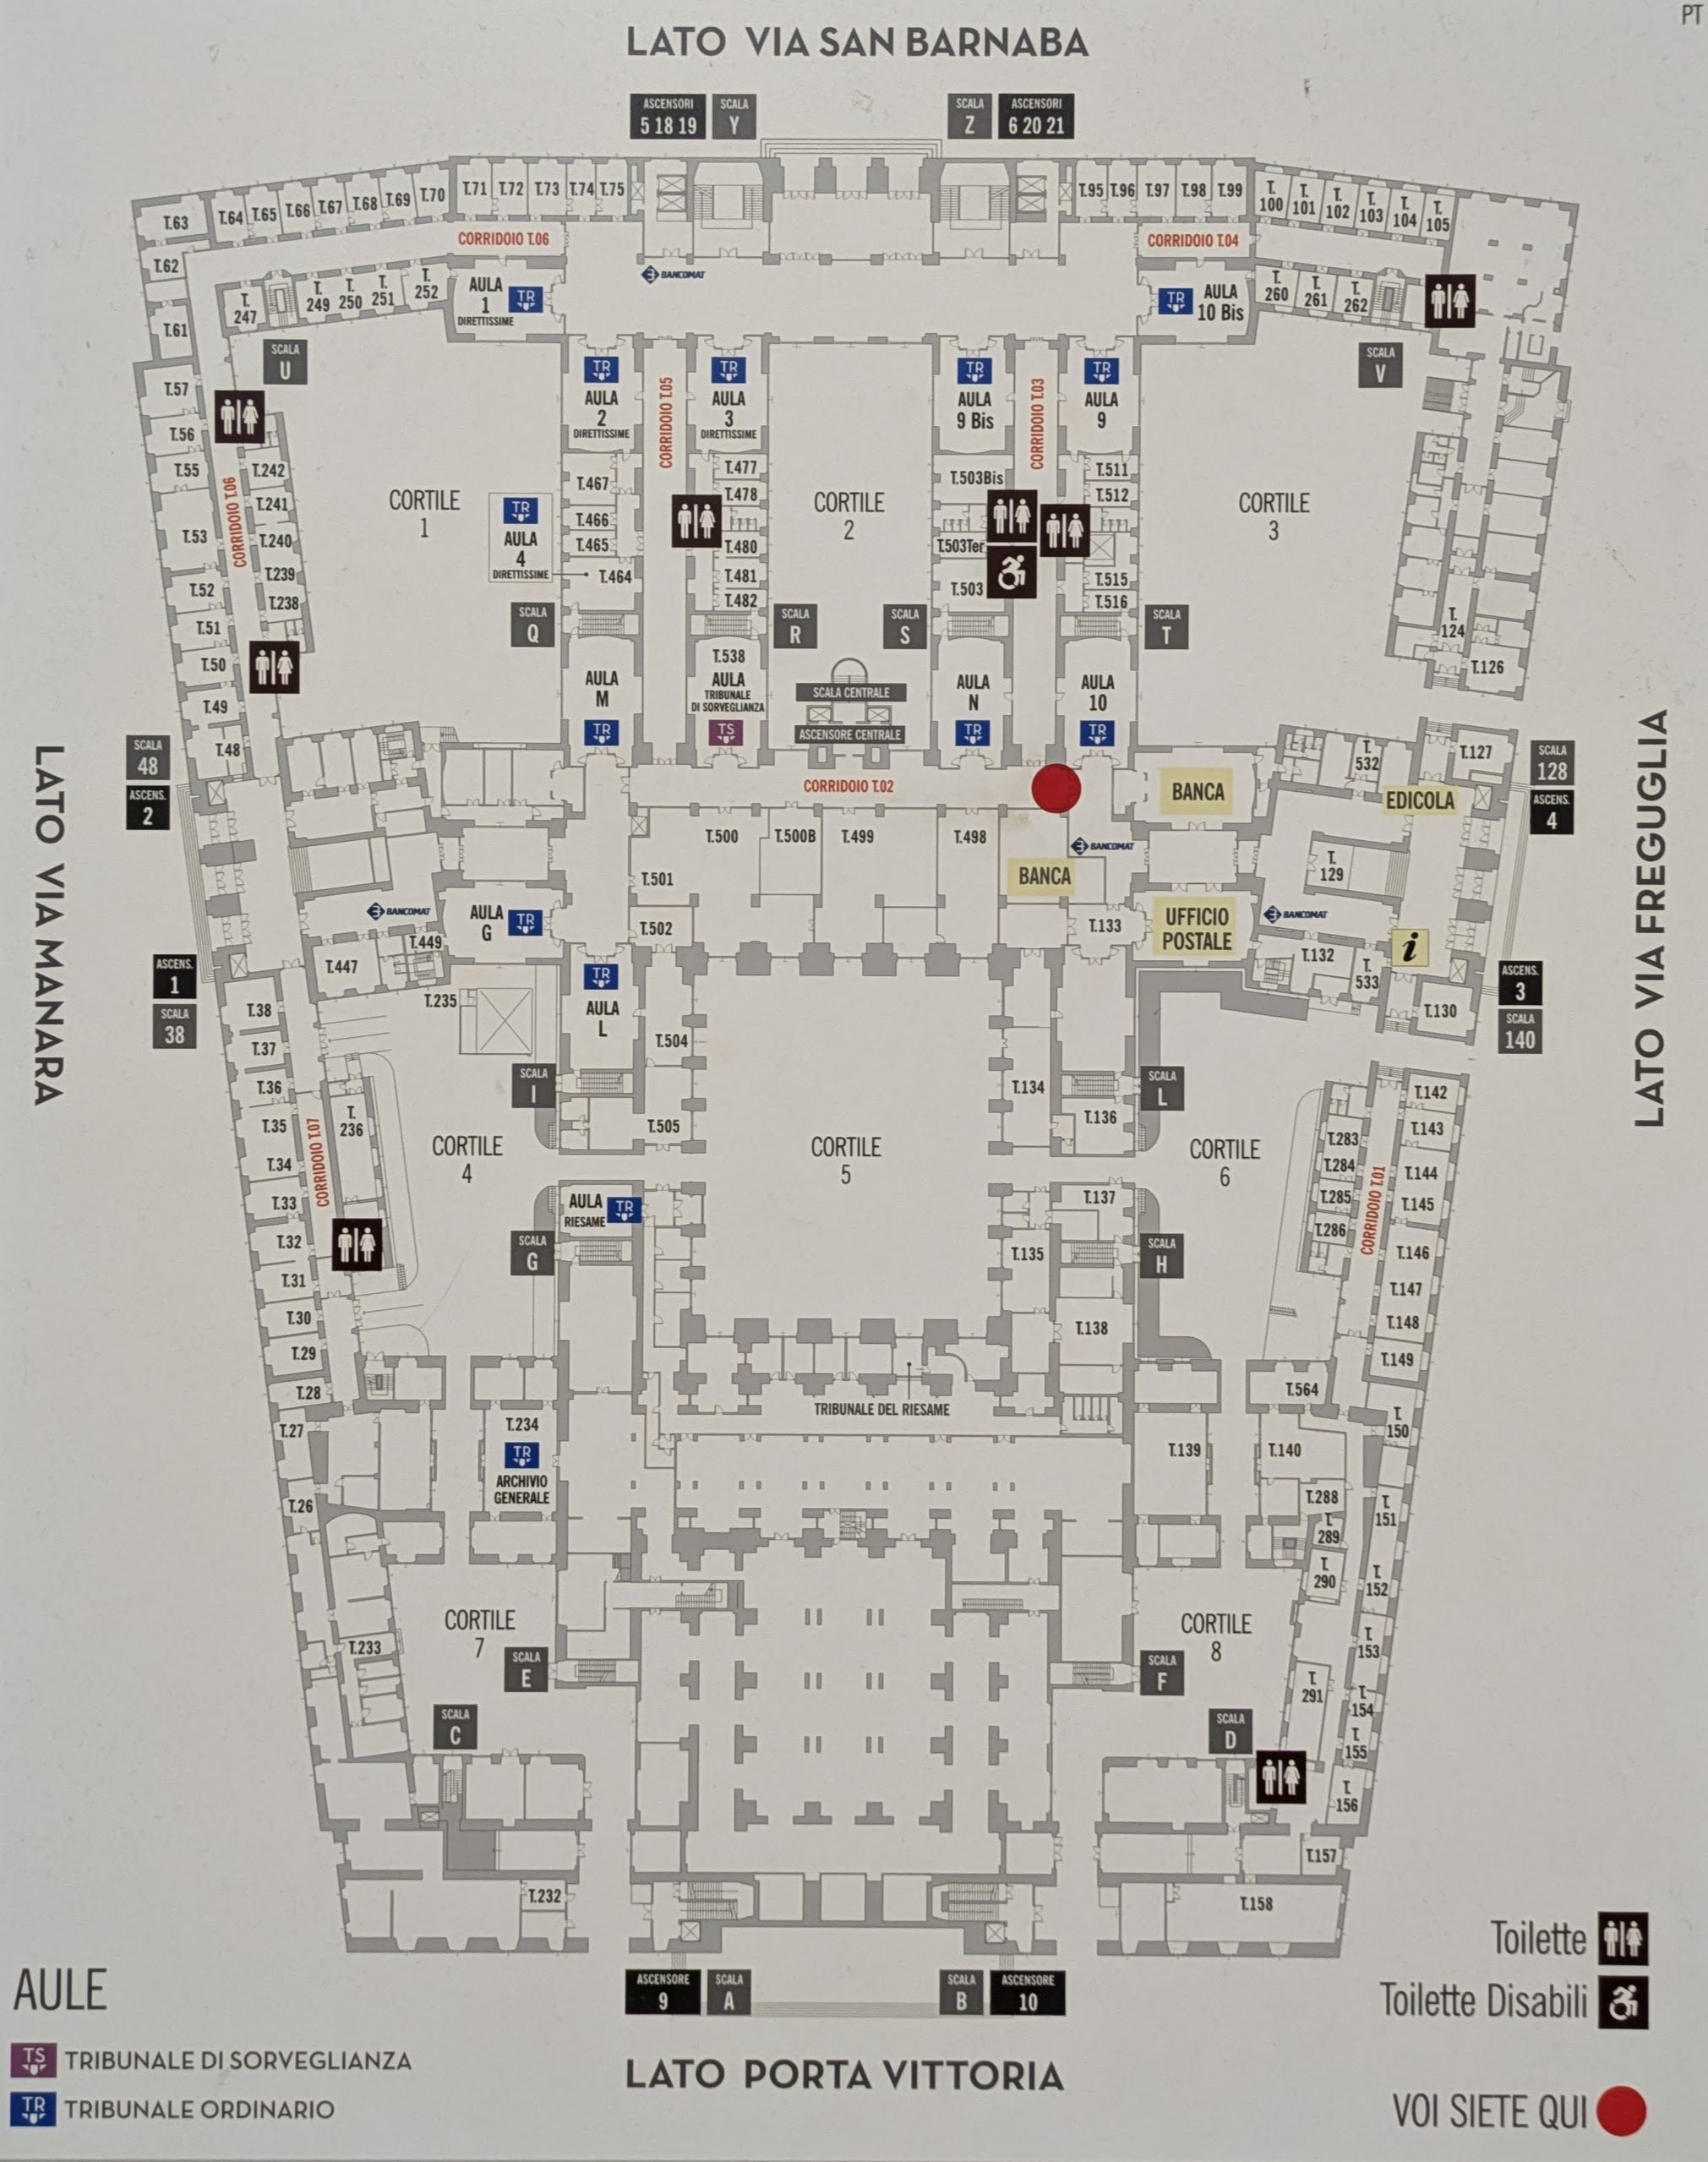
\includegraphics[scale=0.205]{pianta.jpg}
\end{center}

\subsection{Spazi}
L'edificio ha una pianta trapezoidale, presenta 8 cortili interni ed è diviso nel senso longitudinale in tre sezioni:
\begin{itemize}
  \item la Corte d'Appello, lato \textit{Corso di Porta Vittoria}
  \item il Tribunale, lati \textit{via Manara} e \textit{via Freguglia}
  \item la Pretura, lato \textit{via San Barnaba}
\end{itemize}
Ogni sezione ha un proprio ingresso esterno e uno spazio detto \textit{"ambulatorio"}, dal quale si può accedere alle aule della sezione. In totale le aule sono circa 40, e sono presenti anche una biblioteca, un bar e degli uffici. Le sezioni sono collegate internamente da due gallerie longitudinali parallele. \\
Il palazzo presenta quattro piani e due piani ammezzati, e si divide verticalmente nella parte inferiore per i servizi penali e nella parte superiore per quelli civili. \\
Al vertice sud-ovest è invece presente una torre alta 61 metri con 7 piani, che viene impiegata come archivio.

\begin{figure}[h]
  \centering
  \subcaptionbox*{Torre}{%
    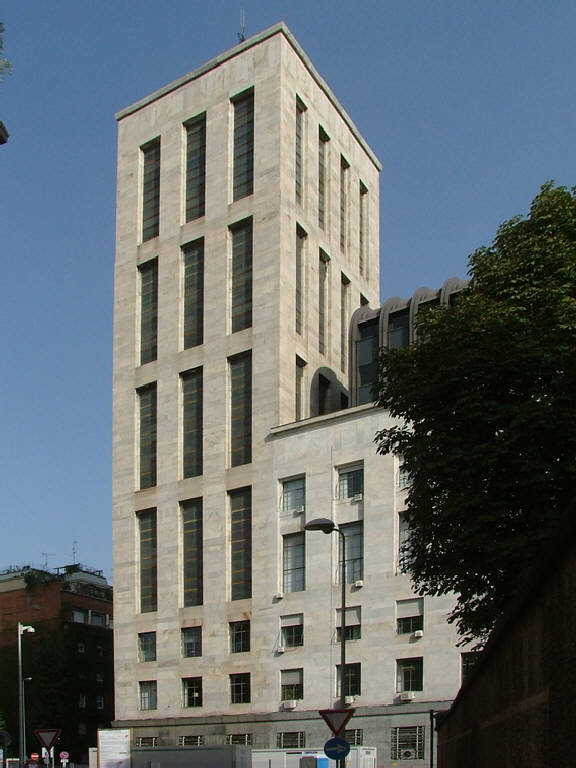
\includegraphics[scale=0.25]{torre.jpg}%
  }\qquad
  \subcaptionbox*{Statua \textit{"La Giustizia"}}{%
    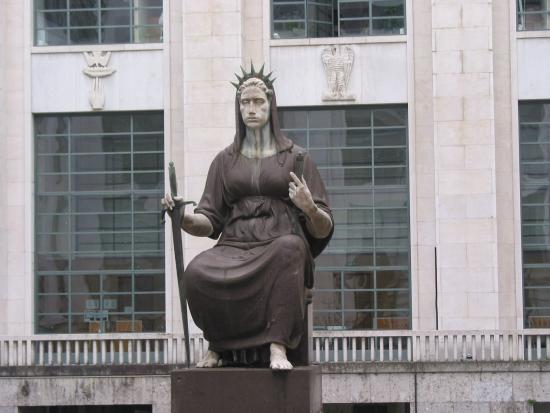
\includegraphics[scale=0.45]{statua.jpg}%
  }
\end{figure}

Nel Cortile d'Onore (numero 5 sulla pianta) è inoltre presente un'imponente statua in porfido e in marmo realizzata da Attilio Selva, intitolata \textit{"La Giustizia"}. 

\newpage
\section{Analisi strutturale}
\subsection{Materiali}
I materiali utilizzati sono:
\begin{itemize}
  \item il calcestruzzo armato per la struttura portante a pilastri
  \item il laterizio forato per le murature d'ambito e la partizione interna
  \item il marmo di Vallestrona per il rivestimento e le pavimentazioni
  \item il serizzo per la zona basamentale della facciata principale
  \item la diorite scura per la grande scalinata frontale
\end{itemize}

\subsection{Collegamenti verticali}
\begin{itemize}
  \item gradinata esterna che precede la facciata principale
  \item 6 scaloni interni e numerose scale secondarie
  \item 9 ascensori
\end{itemize}

\subsection{Prospetti}
% \begin{figure}[h]
%   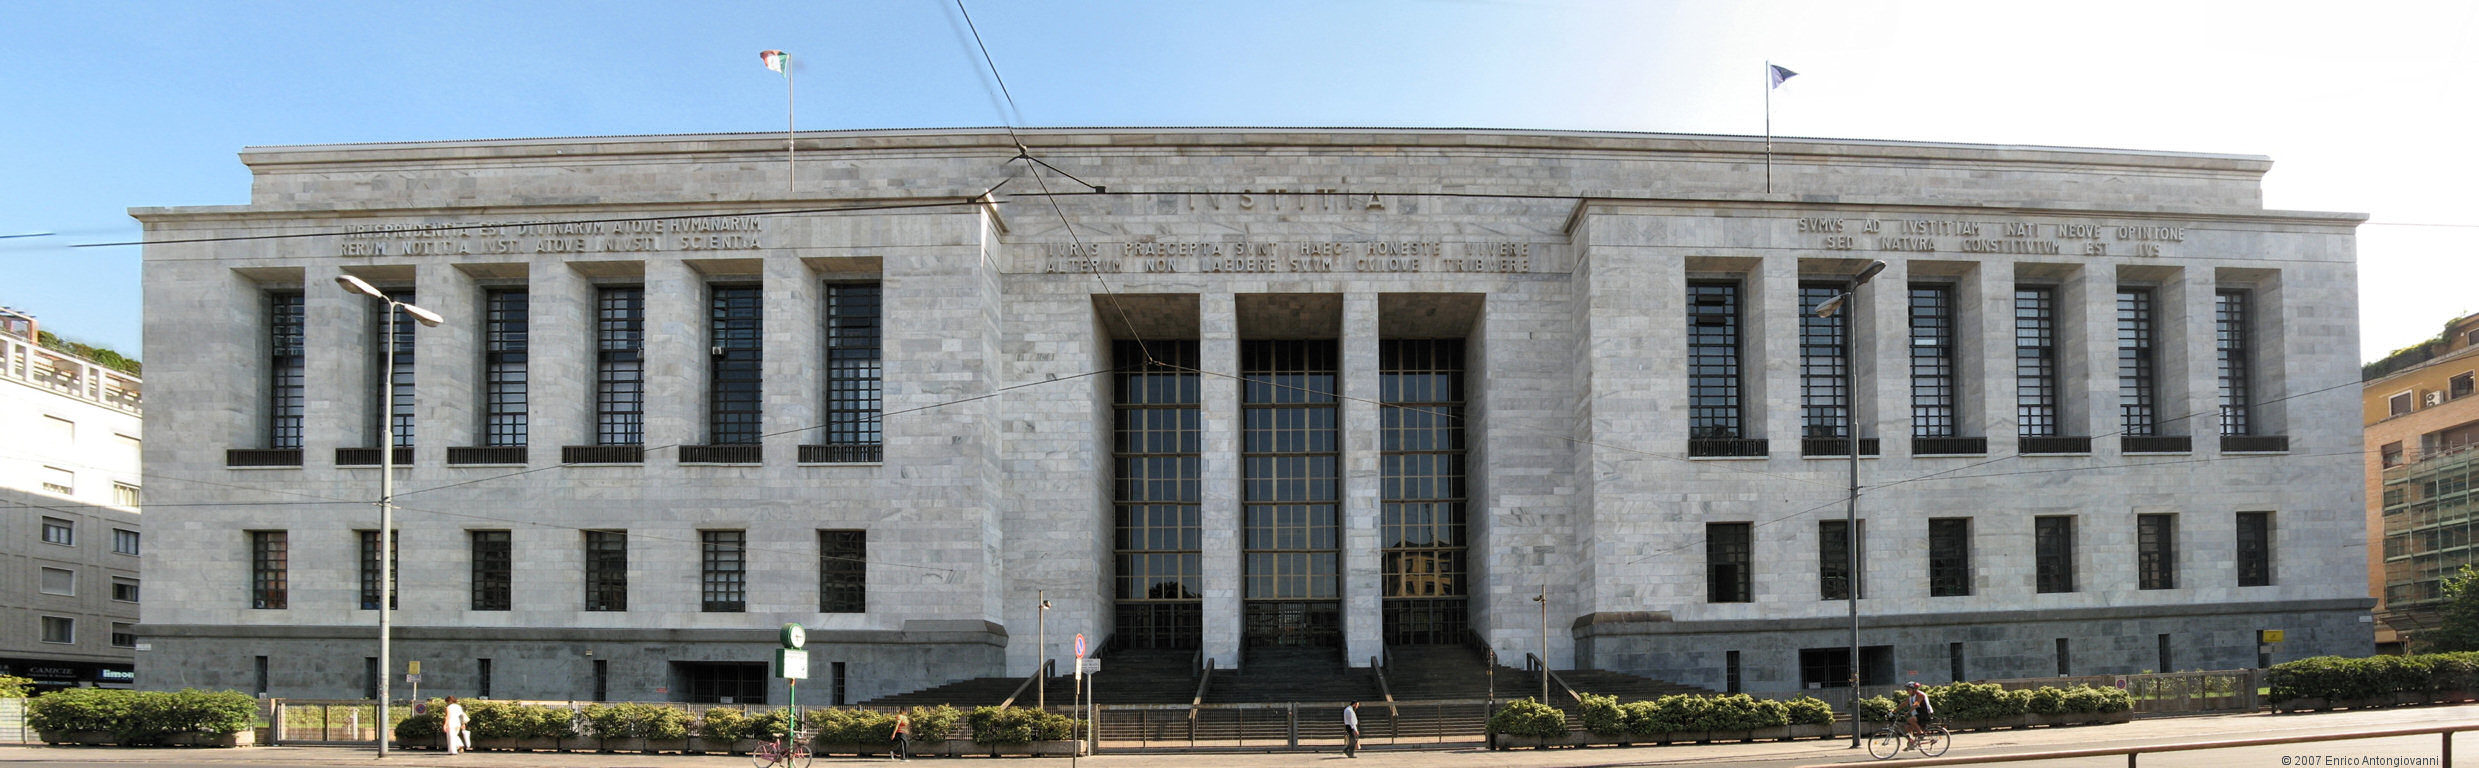
\includegraphics[width=\textwidth]{prospetto_frontale.jpg}
%   \caption*{Prospetto frontale}
% \end{figure}
\subsubsection{Prospetto frontale}
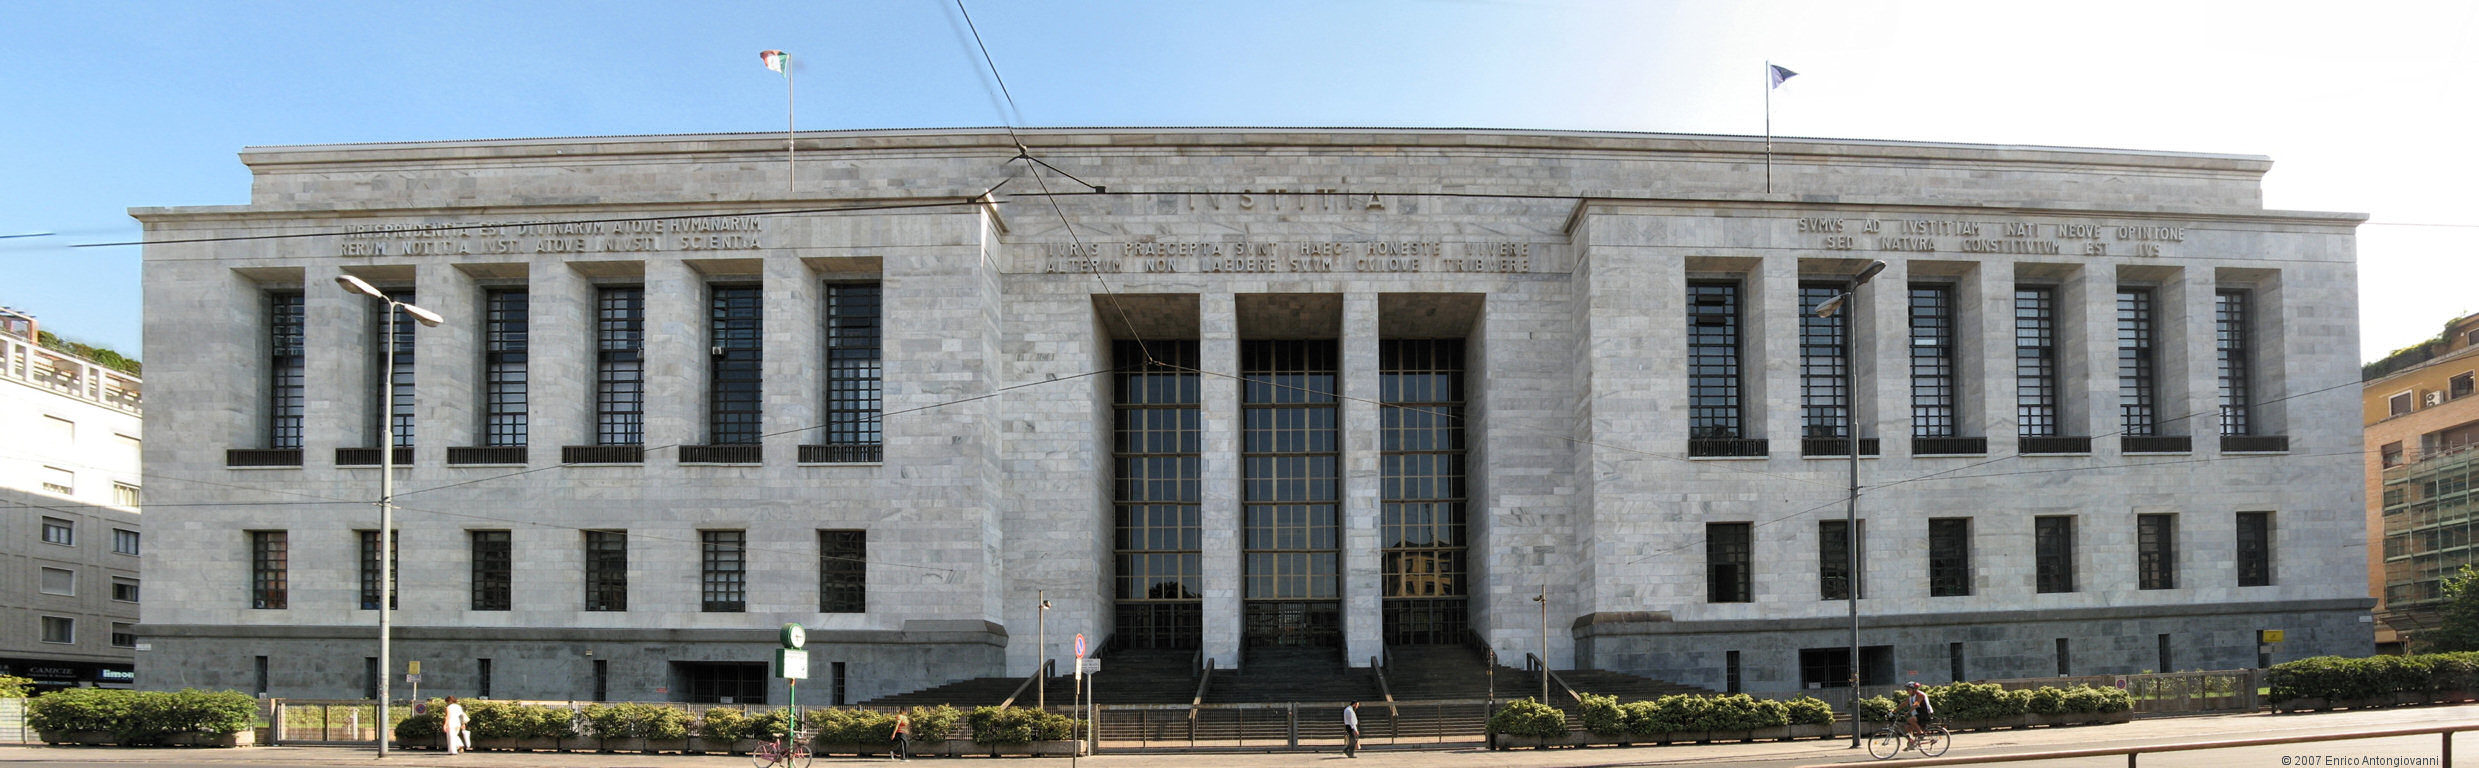
\includegraphics[width=\textwidth]{prospetto_frontale.jpg}
La facciata principale, imponente e austera, è aperta da un triplice portale d'accesso che precede il vestibolo di smistamento. \\
Il portale è alto 25 metri ed è sormontato da un'epigrafe giustinianea, che è l'unico elemento decorativo del coronamento. \\
È inoltre presente una successione a ritmo serrato di finestre alte 8 metri.


\subsubsection{Prospetto laterale su via Manara}
\begin{center}
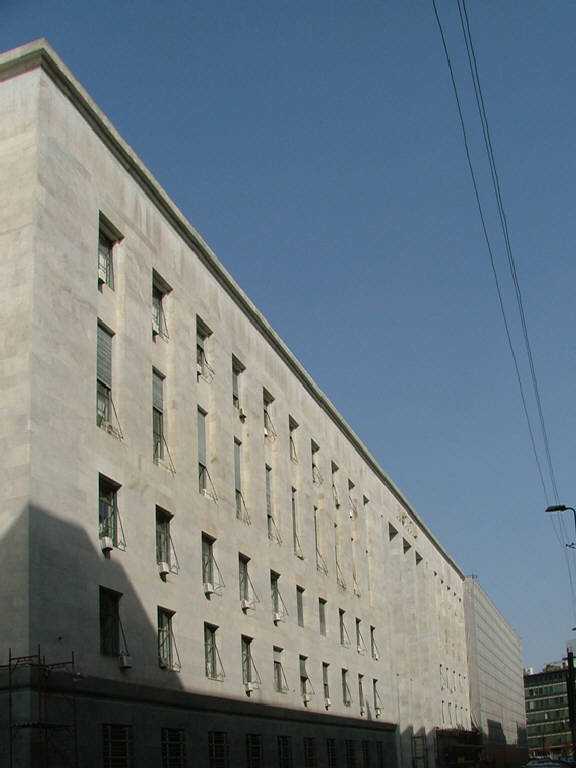
\includegraphics[scale=0.2]{prospetto_manara.jpg}
\end{center}

\subsubsection{Prospetto su via San Barnaba}
\begin{center}
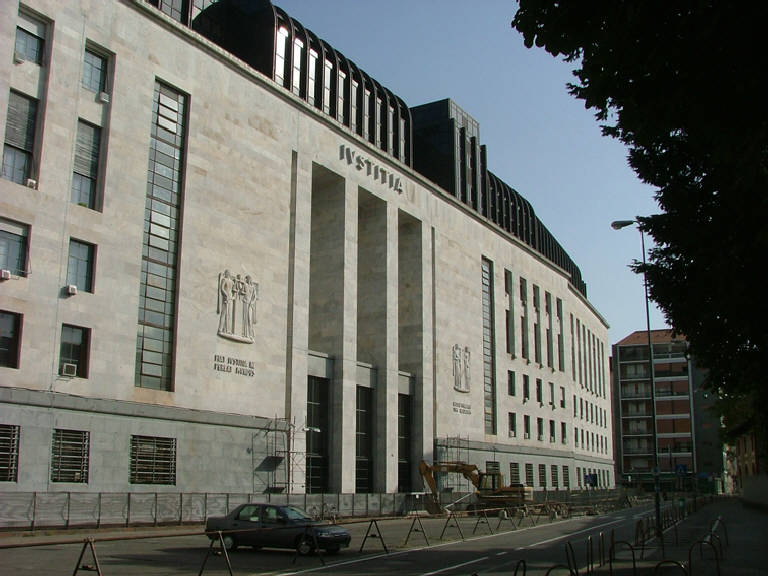
\includegraphics[scale=0.2]{prospetto_barnaba.jpg}
\end{center}

\newpage
\section{Analisi formale}

\newpage
\section{Disegni dei progetti non realizzati}
\subsection{Bianco, rosso e nero}
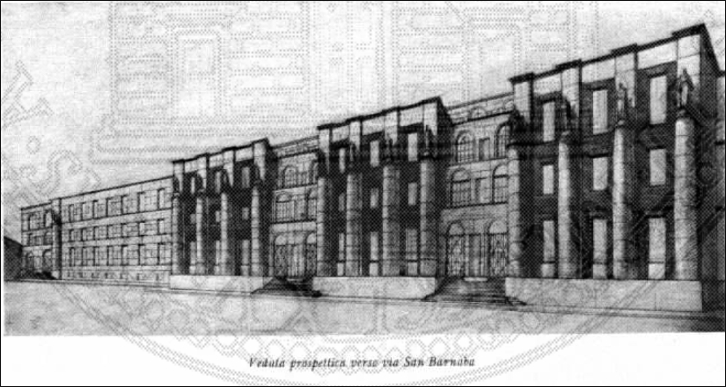
\includegraphics[width=\textwidth]{bianco_rosso_nero2.png}
\begin{center}
  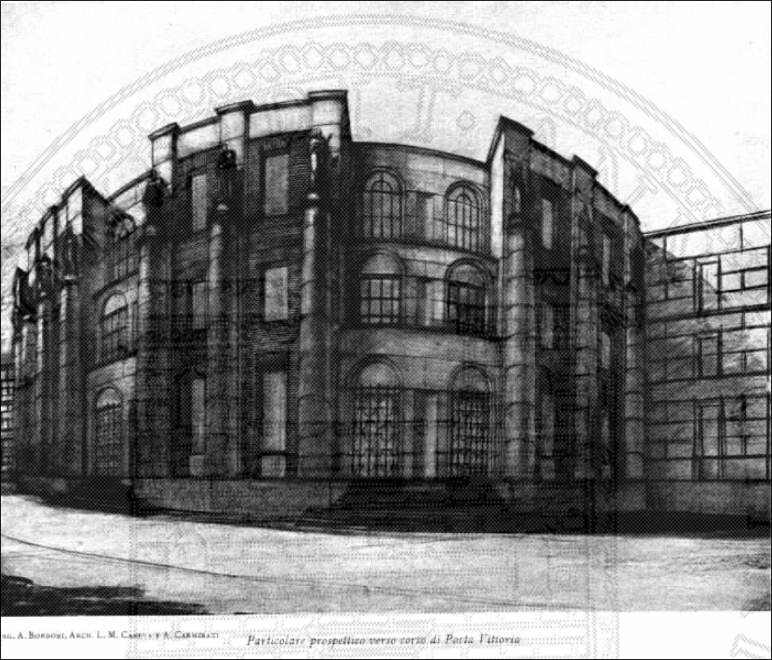
\includegraphics[scale=0.43]{bianco_rosso_nero1.png}
\end{center}

\subsection{Ruit hora}
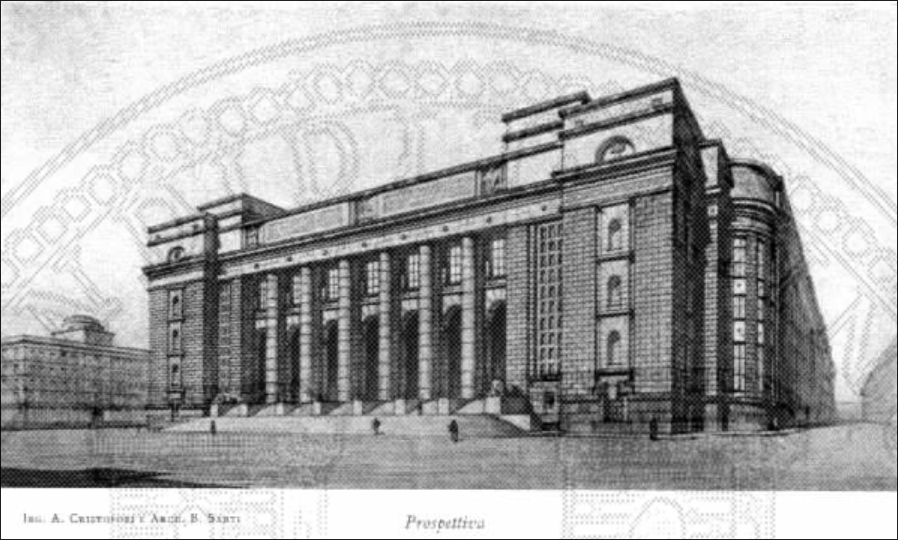
\includegraphics[width=\textwidth]{ruit_hora1.png}

\subsection{Justitia}
\begin{center}
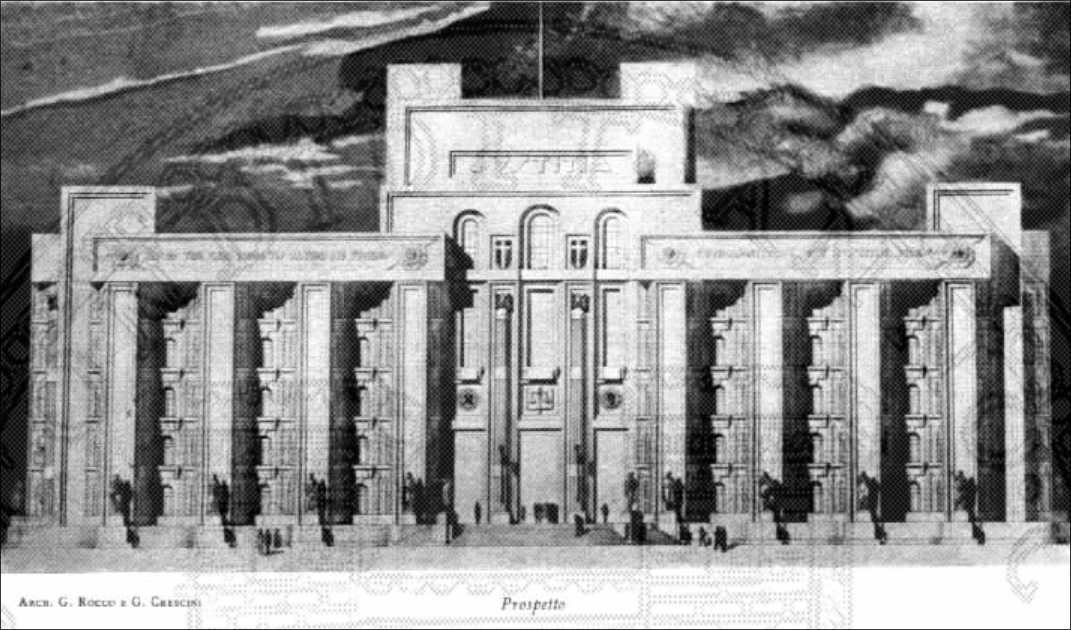
\includegraphics[scale=0.4]{justitia1.png}
\end{center}
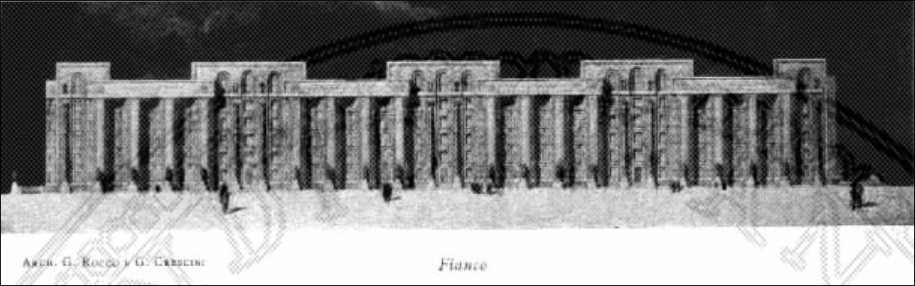
\includegraphics[width=\textwidth]{justitia3.png}

\subsection{Col vento e contro il vento}
\begin{center}
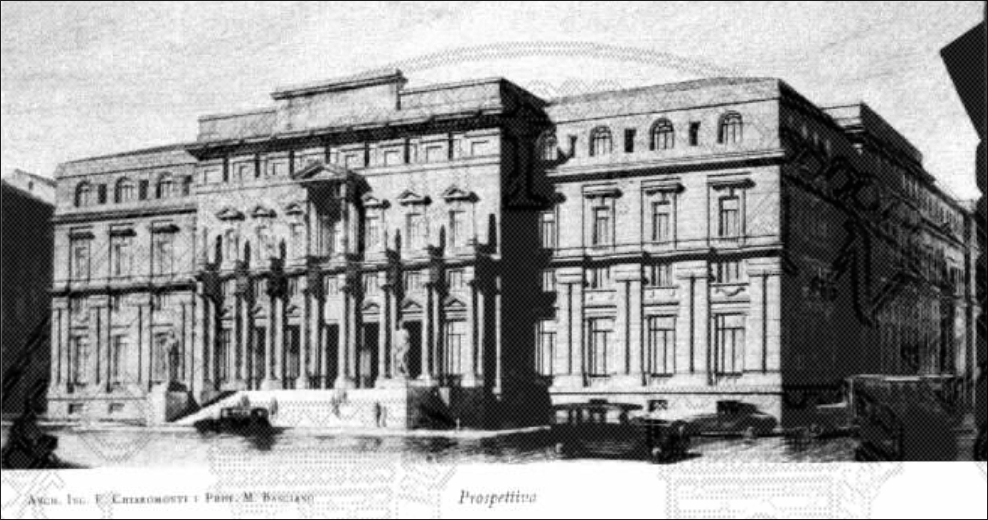
\includegraphics[scale=0.4]{1777662986.png}
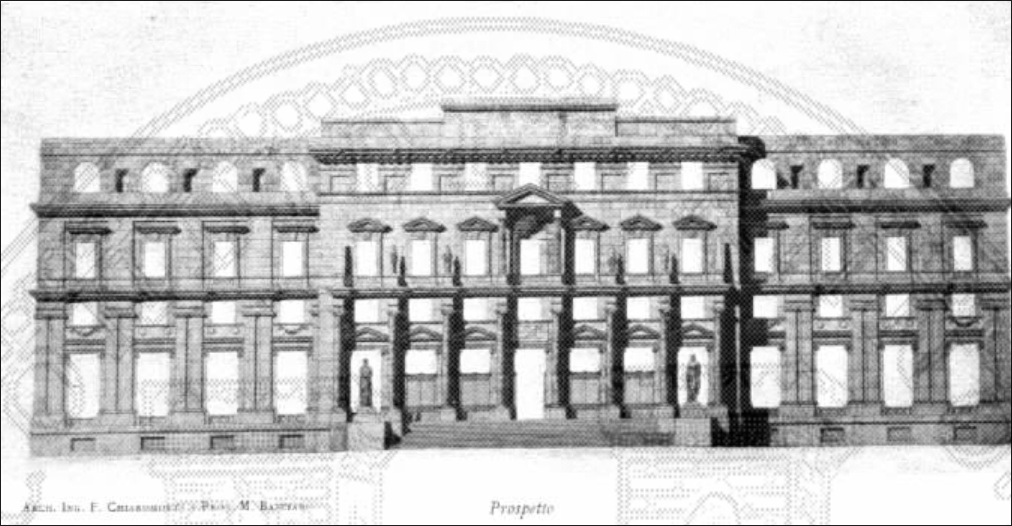
\includegraphics[scale=0.36]{1777661976.png}
\end{center}

\newpage
\section{Fonti}
\begin{itemize}
  \item \url{https://www.lombardiabeniculturali.it/architetture/schede/3m080-00054/}
  \item \url{https://www.lombardiabeniculturali.it/architetture/schede-complete/3m080-00054/}
  \item \url{http://periodici.librari.beniculturali.it/PeriodicoScheda.aspx?id\_testata=22\&Start=0} - periodico numero 5 del 1930
\item \url{https://www.giustiziamilano.it/files/storia-palazzo-giustizia.pdf} - pagine 12, 13, 14, 17, 18, 19
\end{itemize}

\end{document}
